\documentclass[../main/main.tex]{subfiles}
\graphicspath{{./figures/}}

\makeatletter
\renewcommand{\@chapapp}{Travaux pratiques -- TP}
\makeatother

% \toggletrue{student}
\HideSolutionstrue
\toggletrue{corrige}
% \renewcommand{\mycol}{black}
\renewcommand{\mycol}{gray}

\begin{document}
\setcounter{chapter}{7}

\chapter{\cswitch{Correction du TP}{Oscillateurs amortis en \'electricit\'e et
	  m\'ecanique}}

\enonce{
	\begin{prgm}
		\begin{tcb}*(ror)"how"{Savoir-faire}
			\begin{itemize}[label=$\diamond$, leftmargin=10pt]
				\item Mettre en évidence la similitude des comportements des
				      oscillateurs mécanique et électronique.
				\item Réaliser l’acquisition d’un régime transitoire pour
				      un système linéaire du deuxième ordre et analyser ses
				      caractéristiques.
			\end{itemize}
		\end{tcb}
	\end{prgm}
	\vspace{-10pt}
	\section{Objectifs}
	\begin{itemize}
		\item Étudier plus précisément le régime pseudo-périodique d'un circuit RLC
		      peu amorti.
		\item Étudier le comportement d'un oscillateur mécanique vertical amorti
		      avec amortissement faible.
		\item Tracer  une allure de trajectoire de phase correspondant au régime
		      pseudo-périodique.
		\item Vérifier la décroissance exponentielle des amplitudes dans les deux
		      domaines.
		\item Établir un tableau des analogies entre la mécanique et l'électricité.
	\end{itemize}
}

\enonce{
	\section{S'approprier}

	%\subsection{Définition générale d'une trajectoire de phase (hors-programme)}
	%
	%Définition~: On peut décrire l'évolution d'un système quelconque (mécanique ou
	%électrique), pour des conditions initiales données, par la trajectoire dans
	%l'\textbf{espace des phases} $(x \, ; \dot{x})$  ou $(u_{C} \, ; \dot{u_{C}})$
	%ou  plus généralement (variable~; dérivée de la variable) appelée
	%\textbf{trajectoire de phase}. L'ensemble des trajectoires de phase, pour
	%toutes les conditions initiales possibles, est appelé \textbf{portrait de
	%phase}. 

	\subsection{Rappel concernant l'oscillateur mécanique vertical}

	\setlist[blocQR,1]{leftmargin=10pt, label=\clenumi}

	\noindent
	\begin{minipage}[t]{.45\linewidth}
		Soit un oscillateur mécanique vertical (cf.\ Figure~\ref{fig:OH}), constitué
		d'un ressort de raideur $k = \SI{10}{N.m^{-1}}$ et d'une masse $m =
			\SI{200}{g}$. Il est légèrement amorti par frottement fluide dans l'air,
		caractérisé par une force de la forme~: $\vv{f}= - \lambda\vv{v}$.
		\bigbreak
		Dans ce cas, l'équation différentielle (obtenue par projection selon la
		direction verticale $z$ du PFD) de l'oscillateur harmonique amorti peut se
		mettre sous la forme~:
		\[
			\boxed{\ddot{z} + \frac{\lambda}{m} \dot{z} + \frac{k}{m} z = 0}
		\]
	\end{minipage}
	\hfill
	\begin{minipage}[t]{.55\linewidth}
		~
		\vspace{-25pt}
		\begin{center}
			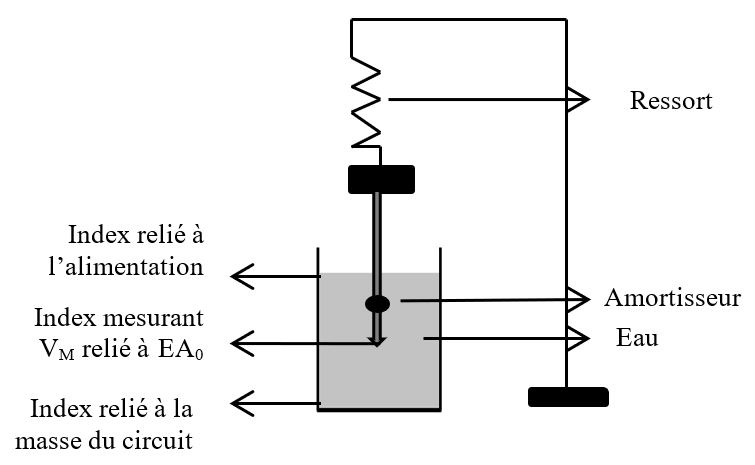
\includegraphics[width=\linewidth]{OH}
			\captionof{figure}{}
			\label{fig:OH}
		\end{center}
	\end{minipage}
}

\QR{%
	Quelle est la période propre attendue~? Peut-on déterminer la pseudo-période
	attendue~?
}{%
	\begin{gather*}
		\w_0 = \sqrt{\frac{k}{m}} = \frac{2\pi}{T_0}
		\\\Lra
		\boxed{T_0 = 2\pi \sqrt{\frac{m}{k}}}
		\qav
		\left\{
		\begin{array}{rcl}
			k & = & \SI{10}{N.m^{-1}}
			\\
			m & = & \SI{0.200}{kg}
		\end{array}
		\right.\\
		\AN
		\xul{
			T_0 = \SI{0.100}{s}
		}
	\end{gather*}
	On ne peut pas déterminer $T$ car il dépend de $Q$ qui dépend de $\lambda$,
	non indiqué.
}

\enonce{
\begin{tcb}(rema){Remarque}
	$z$ est une variable bien choisie pour qu'on ait à l'équilibre $z=0$. C'est
	la raison pour laquelle le poids ainsi que la longueur à vide du ressort
	n'apparaissent pas explicitement dans l'expression.
\end{tcb}

\subsection{Décrément logarithmique}
Pour un régime pseudo-périodique de pulsation $\Omega$, l'amplitude des
oscillations décroît de manière exponentielle~:
\[
	u(t) = u_{\infty} +
	\exr^{- \frac{\w_0}{2Q}t} \times
	\left( A \cos(\Wt) + B\sin(\Wt) \right)
\]
On peut accéder au facteur de
qualité en étudiant le \textbf{décrément logarithmique} $\delta$~:
\[
	\boxed{
	\delta = \frac{1}{n} \ln
	\left( \frac{u(t) - u_{\infty}}{u(t+nT)-u_{\infty}} \right)
	}
\]
avec $n$ le nombre de périodes sélectionnées.
}
\QR{%
	Déterminer la relation entre $\delta$, $\w_0$, $Q$ et $T$ d'abord, puis la
	relation entre $\delta $ et $Q$ uniquement ensuite.
}{%
	\begin{align*}
		u(t+nT) - u_{\infty} & =
		\exr^{- n\frac{\w_0}{2Q}T}\times
		\overbracket[1pt]{\exr^{- \frac{\w_0}{2Q}t}
			\Big(
			A\underset{=\cos\Wt}{\underline{\cos(\W(t+nT))}} +
			B\underset{=\sin\Wt}{\underline{\sin(\W(t+nT))}}
			\Big)
		}^{= u(t) - u_{\infty}}
		\\\Lra
		u(t+nT) - u_{\infty} & =
		\exr^{-n \frac{\w_0}{2Q}T}
		\left( u(t) - u_{\infty} \right)
	\end{align*}
	\vspace{-15pt}
	\begin{gather*}
		\Ra
		\delta = \frac{1}{n}\ln
		\Bigg(
		\frac{\cancel{u(t)-u_{\infty}}}
		{\exr^{-n\frac{\w_0}{2Q}T}\left(\cancel{ u(t) - u_{\infty} }\right)}
		\Bigg) =
		\frac{1}{n}\ln \left( \exr^{n \frac{\w_0}{2Q}T} \right)
		\\\Lra
		\delta = \frac{\w_0}{2Q}T
		\Lra
		\boxed{\delta = \frac{2\pi}{\sqrt{4Q^2-1}}}
	\end{gather*}
}

\setcounter{section}{2}
\section{Analyser~: régime pseudo-périodique du RLC série}

\QR{%
	Faire le schéma d'un circuit RLC série alimenté par une tension
	$e(t)$. On veut visualiser à l'oscilloscope simultanément $e(t)$ sur la
	voie 1 et $u_{C}(t)$ sur la voie 2~: indiquer les connexions de
	l'oscilloscope à réaliser et positionner la masse sur le circuit.
}{%
	\begin{center}
		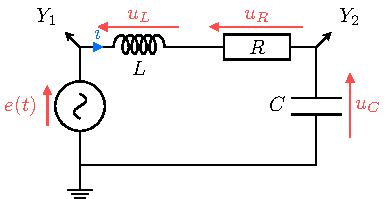
\includegraphics[scale=1]{circ_rlc-start}
		\captionof{figure}{}
	\end{center}
}

\enonce{%
	$e(t)$ est une tension créneau de fréquence $\SI{100}{Hz}$, $C$ une
	boite de capacités. On prendra $C = \SI{0,01}{\micro F}$. $L$ est une
	bobine d'inductance $L= \SI{0,1}{H}$.
}

\QR{%
	Écrire l'équation différentielle en $u_{C}(t)$, puis celle en $q(t) = C
		u_{C}(t)$ et calculer la valeur $R_{c}$ à donner à $R$ pour visualiser le
	régime critique.
}{%
	solu
}
\QR{%
	\label{q:reglin}
	En vous basant sur la Section~II.A., quelle régression linéaire peut-on
	étudier pour obtenir le facteur de qualité~? Exprimer le coefficient directeur
	en fonction de $a$.
	\begin{tcb}*[aide](expe)<itc>{Aide}
		La variable $x$ doit être $nT$.
	\end{tcb}
}{%
	On peut tracer
	\[
		y\tikzmark{yn} = a\tikzmark{an}x\tikzmark{xn} + b\tikzmark{bn}
	\]
	\tikz[remember picture, overlay]
	\draw[-stealth, transform canvas={xshift=-6pt, yshift=-6pt}]
	(pic cs:yn) --++ (-10pt,-10pt)
	node[anchor=north east] {$n\delta$}
	;
	\tikz[remember picture, overlay]
	\draw[-stealth, transform canvas={xshift=-5pt, yshift=-6pt}]
	(pic cs:an) --++(-5pt,-10pt)
	node[anchor=north] {$\frac{\w_0}{2Q}$}
	;
	\tikz[remember picture, overlay]
	\draw[-stealth, transform canvas={xshift=0pt, yshift=-6pt}]
	(pic cs:xn) --++(5pt,-10pt)
	node[anchor=north] {$nT$}
	;
	\tikz[remember picture, overlay]
	\draw[-stealth, transform canvas={xshift=3pt, yshift=-6pt}]
	(pic cs:bn) --++(10pt,-10pt)
	node[anchor=north west] {$0$}
	;
	\noindent
	\bigbreak
	On a alors
	\[
		\boxed{a = \frac{\delta}{T}}
	\]
}

\section{Réaliser et valider}

\subsection{Étude expérimentale du régime pseudo-périodique du RLC}

Réaliser le montage vu précédemment dans l'analyse en prenant les mêmes valeurs
de $e(t)$, $C$ et $L$ que ci-dessus.

\subsubsection{Visualisation et mesure de la pseudo-période}

\begin{tcb}(expe){}
	\begin{enumerate}
		\item Faire varier $R$ de façon à observer un régime pseudo-périodique très
		      peu amorti. Il faut observer au moins une dizaine de maxima successifs
		      sur l'oscillogramme.
	\end{enumerate}
\end{tcb}
\enonce{%
	Dans le cas d'un amortissement très faible, on peut assimiler la
	pseudo-période des oscillations $T$ à la période propre $T_0$ du
	circuit.
}
\resetQ
\setlist[blocQR,1]{leftmargin=10pt, label=\sqenumi}
\QR{%
	Mesurer expérimentalement la pseudo-période $T$ en prenant
	plusieurs périodes pour gagner en précision. La comparer à la période
	propre théorique en calculant l'écart normalisé entre les deux
	grandeurs.
}{%
	On mesure
	\begin{gather*}
		T_1 = \SI{0.50 \pm 0.05}{s}
		\qet
		T_4 = \SI{2.50 \pm 0.05}{s}
		\\\Ra
		\boxed{T_{\exp} = \frac{T_4 - T_1}{4}}
		\qet
		u(T_{\exp}) = \frac{u(T_{1})\sqrt{2}}{4}
		\\\Ra
		\xul{T_{\exp} = \SI{0.50 \pm 0.02}{s}}
	\end{gather*}
	Or,
	\begin{gather*}
		\boxed{T_{\rm theo} = 2\pi \sqrt{LC}}
		\qav
		\left\{
		\begin{array}{rcl}
			L & = & \SI{0.1}{H}
			\\
			C & = & \SI{0.01}{\micro F}
		\end{array}
		\right.\\
		\AN
		\xul{
			T_{\rm theo} = \SI{2.0e-4}{s}
		}
		\\\Ra
		\boxed{E_N = \frac{\abs{T_{\exp} - T_{\rm theo}}}{T_{\rm theo}}}
		\\
		\AN
		\xul{E_N = \num{0.3}}
	\end{gather*}
	Ce qui est acceptable.
}
\QR{%
	Imprimer la courbe obtenue en tenant compte des consignes indiquées
	sur les fiches plastifiées.
}{%
	solu
}

\subsubsection{Décroissance exponentielle de l'amplitude}

Activité \texttt{Capytale} disponible\ftn{3e47-2247217}.
\begin{tcb}(expe){}
	\begin{isd}[righthand ratio=.35]
		\begin{enumerate}
			\item Grâce au curseur horizontal de l'oscilloscope, déterminer
			      $u_{\infty}$ et relever les valeurs des amplitudes successives
			      $u_{C,\max}$ en fonction du nombre de périodes $nT$. Remplir le
			      tableau ci-contre.
			\item Rentrer vos valeurs expérimentales sur \texttt{Capytale}.
			      Créer la variable \texttt{delta\_list} calculant $\delta$ pour
			      chaque itération. Compléter le Tableau~\ref{tab:deltauc}.
			\item Créer la variable nécessaire et effectuer la régression linéaire
			      déterminée à la question~\ref{q:reglin}. Tracer la régression.
		\end{enumerate}
		\tcblower
		\begin{center}
			\captionof{table}{}
			\label{tab:deltauc}
			\begin{tabular}{lccc}
				\toprule
				$n$      & $nT$     & $u_{c, \max}$ & $\delta $ \\
				\midrule
				0        & $\ldots$ & $\ldots$      & $\ldots$  \\
				1        & $\ldots$ & $\ldots$      & $\ldots$  \\
				2        & $\ldots$ & $\ldots$      & $\ldots$  \\
				3        & $\ldots$ & $\ldots$      & $\ldots$  \\
				4        & $\ldots$ & $\ldots$      & $\ldots$  \\
				$\vdots$ & $\vdots$ & $\vdots$      & $\vdots$  \\
				\bottomrule
			\end{tabular}
		\end{center}
	\end{isd}

\end{tcb}

\QR{%
	Quel est le coefficient directeur $a_{\exp}$ de la droite obtenue~? Quel est
	donc le facteur de qualité $Q_{\exp}$ obtenu~?
	Donner l'expression de $Q_{\rm theo}$, en fonction de $R$, $C$ et
	$L$. Calculer l'écart normalisé. Commenter.
}{%
	\leftcenters{%
		On obtient
	}{%
		$\DS a_{\exp} = \SI{0.314}{rad.s^{-1}} = \frac{\w_0}{2Q}$
	}
	\smallbreak
	\leftcenters{%
		Ainsi,
	}{%
		$Q_{\exp} = \frac{\pi}{a_{\exp}T}
			\qquad \Ra \qquad
			\xul{Q_{\exp} = \num{15}}$
	}
	\smallbreak
	\leftcenters{%
		Or,
	}{%
		$\DS Q_{\rm theo} = \frac{1}{R} \sqrt{\frac{L}{C}}
			\qquad \Ra \qquad
			\xul{Q_{\rm theo} = \SI{0.314}{rad.s^{-1}}}$
	}
	\smallbreak
	\leftcenters{%
		Ainsi
	}{%
		$E_N = \frac{\abs{Q_{\exp} - Q_{\rm theo}}}{Q_{\rm theo}} = \num{0.3}$
	}
	\smallbreak
	C'est tout à fait acceptable.
}

\subsection{Étude expérimentale d'oscillations mécaniques amorties}

\subsubsection{Montage expérimental}

Le montage est schématisé dans la partie S'approprier, et est déjà réalisé. On
mesure une tension sur la voie $EA0$ qui est proportionnelle à l'ordonnée $z$ du
point matériel de masse $m$.
\begin{tcb}[cnt, bld](impo){}
	La masse $m$ ne doit pas toucher à l'eau de l'éprouvette.
\end{tcb}

\subsubsection{Réglages de l'ordinateur}

\begin{tcb}[breakable](expe){}
	\begin{enumerate}
		\item Avant tout réglage~: brancher l'interface SYSAM et l'alimentation
		      stabilisée sur $\SI{7}{V}$.
		\item Ouvrir latispro (programmes $\ra$ discipline $\ra$ physique-chimie
		      $\ra$ eurosmart $\ra$ latispro).
		\item Pour faire une acquisition~: bouton
		      
\includegraphics[width=0.05\textwidth]{bouton_acq}
		\item Pour activer la voie $EA0$~:
		      \begin{itemize}
			      \item Dans le cadre \textit{entrées analogiques}, cliquer sur les
			            boutons des entrées à activer.
			      \item Cliquer droit et choisir \textit{trait}.
		      \end{itemize}
		\item Pour paramétrer l'acquisition~:
		      \begin{itemize}
			      \item Dans le cadre acquisition, onglet temporel, mode normal,
			            entrer le nombre de points de mesure et la durée totale de
			            l'acquisition.
			      \item Acquisition temporelle~; durée~: $\SI{30}{s}$~; nombre de
			            points~: 2000.
		      \end{itemize}
		\item Fin des réglages~! Vous êtes prêt-es à faire vos enregistrements.
	\end{enumerate}
\end{tcb}

\subsubsection{Mesures}

\begin{tcb}(expe){}
	\begin{enumerate}
		\item Lorsque la position est à sa position d'équilibre, le bout du fil doit
		      être au milieu du bécher. Si ce n'est pas le cas, modifier la hauteur du
		      point d'attache du ressort.
		\item Étirer légèrement le ressort sans qu'il ne touche au fond du bécher.
		\item Lorsque les oscillations paraissent régulières, lancer l'acquisition
		      en cliquant sur 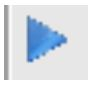
\includegraphics[width=0.03\textwidth]{bouton_go}.
	\end{enumerate}
\end{tcb}

\subsubsection{Exploitation des résultats}

\enonce{%
	Dans le cas d'un amortissement très faible, on peut assimiler la
	pseudo-période des oscillations $T$ à la période propre $T_0$ du circuit.
}
\QR{%
	Grâce au réticule (cliquer droit et choisir), mesurer expérimentalement la
	pseudo-période $T$ en prenant plusieurs périodes pour gagner en précision. La
	comparer à la période propre théorique en calculant l'écart normalisé entre
	les deux grandeurs.
}{%
	solu
}

\begin{tcb}(expe){}
	\begin{enumerate}
		\item Grâce au réticule (lié à la courbe pour plus de facilité), relever les
		      valeurs des amplitudes successives $u_{\max}$ en fonction du nombre de
		      périodes $nT$ (environ 15 mesures)~; cliquer droit, puis calibrage pour
		      modifier l'échelle.

		\item Créer le tableau de valeurs $(nT~; u_{\max})$ correspondant
		      (cf.\ Tableau~\ref{tab:deltauc}), que vous recopierez sur vos copies.

		\item Créer la variable nécessaire de façon à vérifier que l'amplitude
		      des oscillations décroit de façon exponentielle, et la modéliser par une
		      droite.
	\end{enumerate}
\end{tcb}

\QR{%
	Quel est le coefficient directeur $a_{\exp}$ de la droite obtenue~?
	Grâce aux relations vues en cours, en
	déduire un ordre de grandeur du coefficient d'amortissement $\lambda$.
}{%
	solu
}
\QR{%
	Imprimer la courbe obtenue ainsi que sa modélisation.
}{%
	solu
}

%\medskip
%
%\underline{Tracé d'une trajectoire de phase}~:
%
%\begin{itemize} \item Créer la variable dérivée nécessaire au tracé de la
%trajectoire de phase~: $deriv(EA0 \, ; \, t)$~: dérivée du signal de la voie
%$EA0$ par rapport au temps $t$. \item Tracer la trajectoire de phase grâce aux
%choix d'abscisses et d'ordonnées dans les options de graphe. Imprimer la
%courbe. Quelle est l'allure de la courbe obtenue~? Commenter qualitativement.
%Intuiter l'allure s'il n'y avait aucun amortissement. \end{itemize}

\section{Conclure}

\QR{%
	Quelles similitudes de comportements entre les deux types d'oscillateurs ont été
	observées~? En utilisant les études théoriques demandées (équations
	différentielles), ainsi que les résultats expérimentaux trouvés, recopier et
	compléter le tableau suivant~:
	\captionof{table}{Correspondances}
	\centering
	\begin{tabular}{c@{$\longleftrightarrow$}c}
		\toprule
		Méca                                  & Élec
		\\
		\midrule
		$z$                                   & $q$
		\\
		\wht{$v$}                             & $i$
		\\
		\wht{$m$}                             & $L$
		\\
		\wht{$k$}                             & $C$
		\\
		\wht{$\sqrt{\frac{k}{m}}$}            & $\w_0 = \frac{1}{\sqrt{LC}}$
		\\
		\wht{$\lambda$}                       & $R$
		\\
		\wht{$Q = \frac{\sqrt{km}}{\lambda}$} & $Q = \frac{1}{R}\sqrt{\frac{L}{C}}$
		\\
		\bottomrule
	\end{tabular}
}{%
	\captionof{table}{Correspondances}
	\centering
	\begin{tabular}{c@{$\longleftrightarrow$}c}
		\toprule
		Méca                            & Élec
		\\
		\midrule
		$z$                             & $q$
		\\
		$v$                             & $i$
		\\
		$m$                             & $L$
		\\
		$k$                             & $C$
		\\
		$\sqrt{\frac{k}{m}}$            & $\w_0 = \frac{1}{\sqrt{LC}}$
		\\
		$\lambda$                       & $R$
		\\
		$Q = \frac{\sqrt{km}}{\lambda}$ & $Q = \frac{1}{R}\sqrt{\frac{L}{C}}$
		\\
		\bottomrule
	\end{tabular}
}

\end{document}
